
\subsubsection{Electric polarizability $\alpha_E$ including all diagrams in the 3-window analysis}
\label{3573wAll}
The 3-window analysis was also performed for all diagrams, connected and disconnected,
shown in~\ref{fig:diagrams}. The correlator ratios $R_2(t)$ are shown in figure~\ref{fig:Correlators3wAll}. 
The plots roughly correspond to the cubic behavior depicted in~\ref{fig:CubicAll}.
 The inflection points and extremal slopes were obtained for 
 the fitting ranges 5 to 7, 4 to 8, 3 to 9, as shown in~\ref{tab:ExtremaMultiPointAll}.
%%%%%%%%%All diagrams R(t)%%%%%%
\begin{figure}[H]
\centering
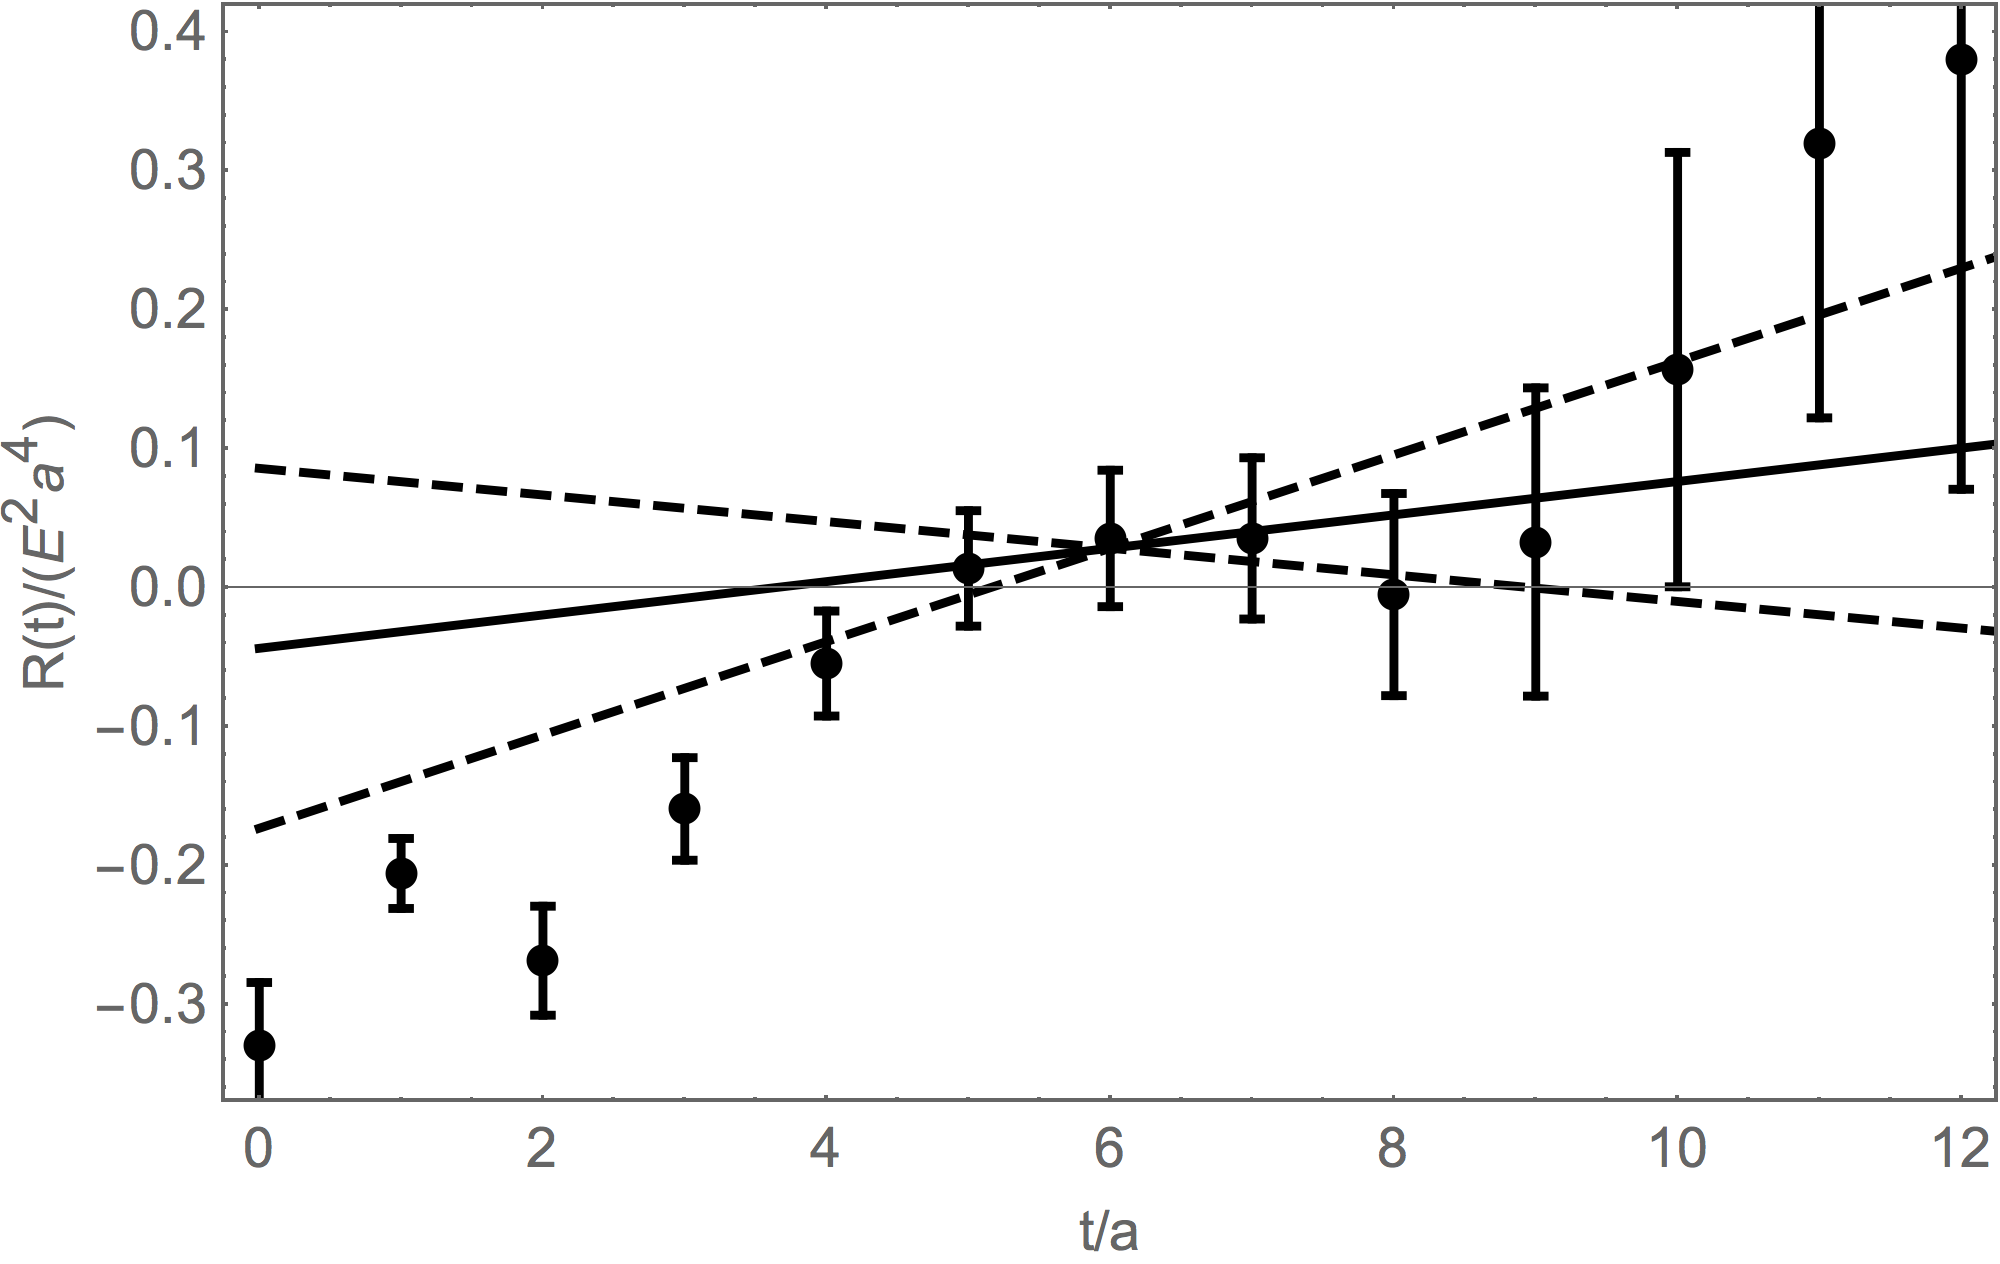
\includegraphics[width=.333\linewidth]{figures/FullshshLineCS.png}
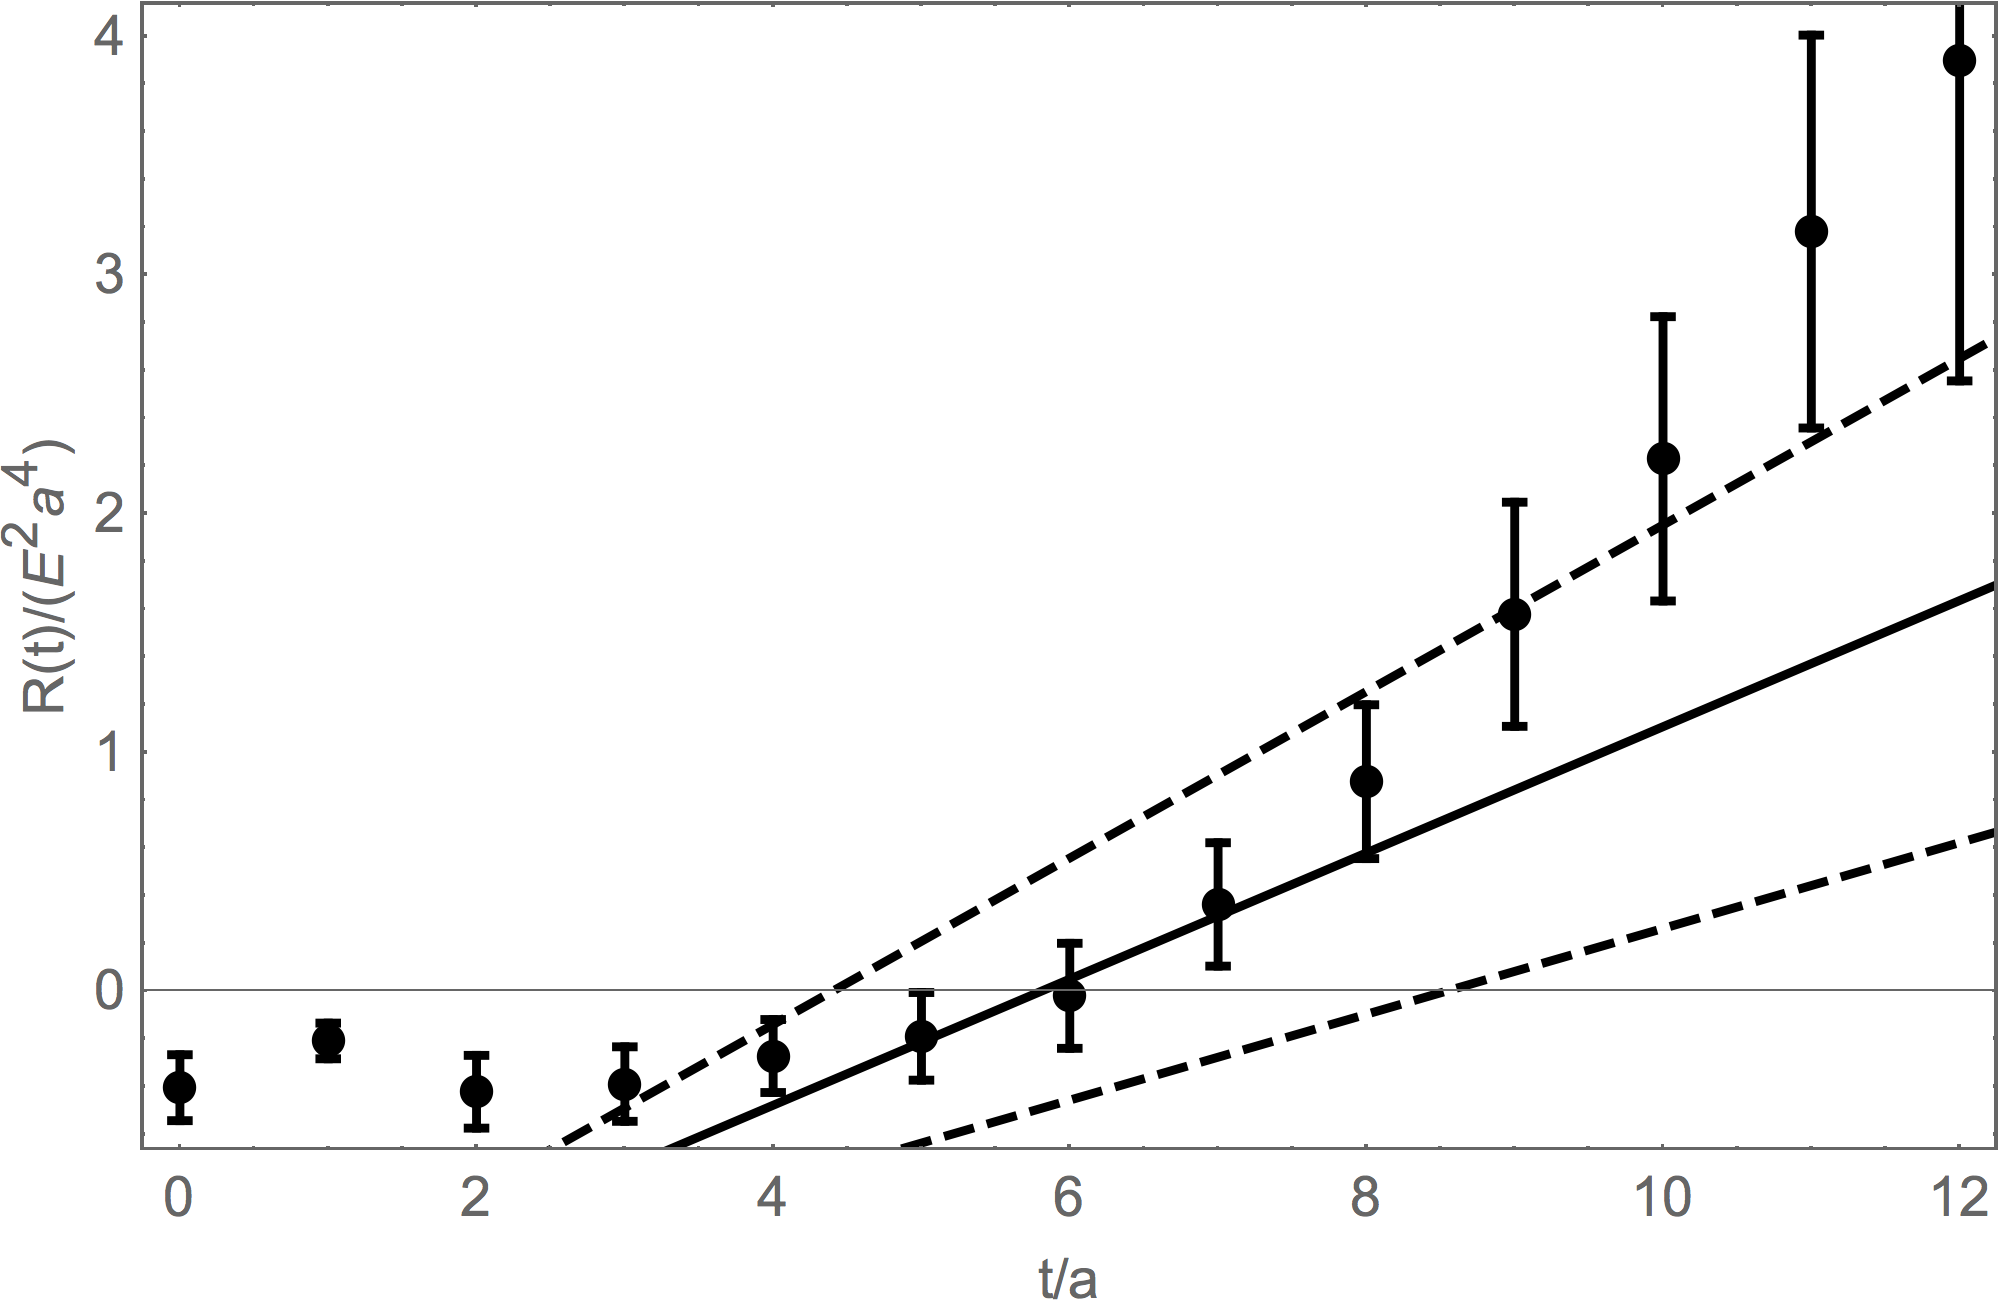
\includegraphics[width=.32\linewidth]{figures/Fullfrom0LineCS.png}
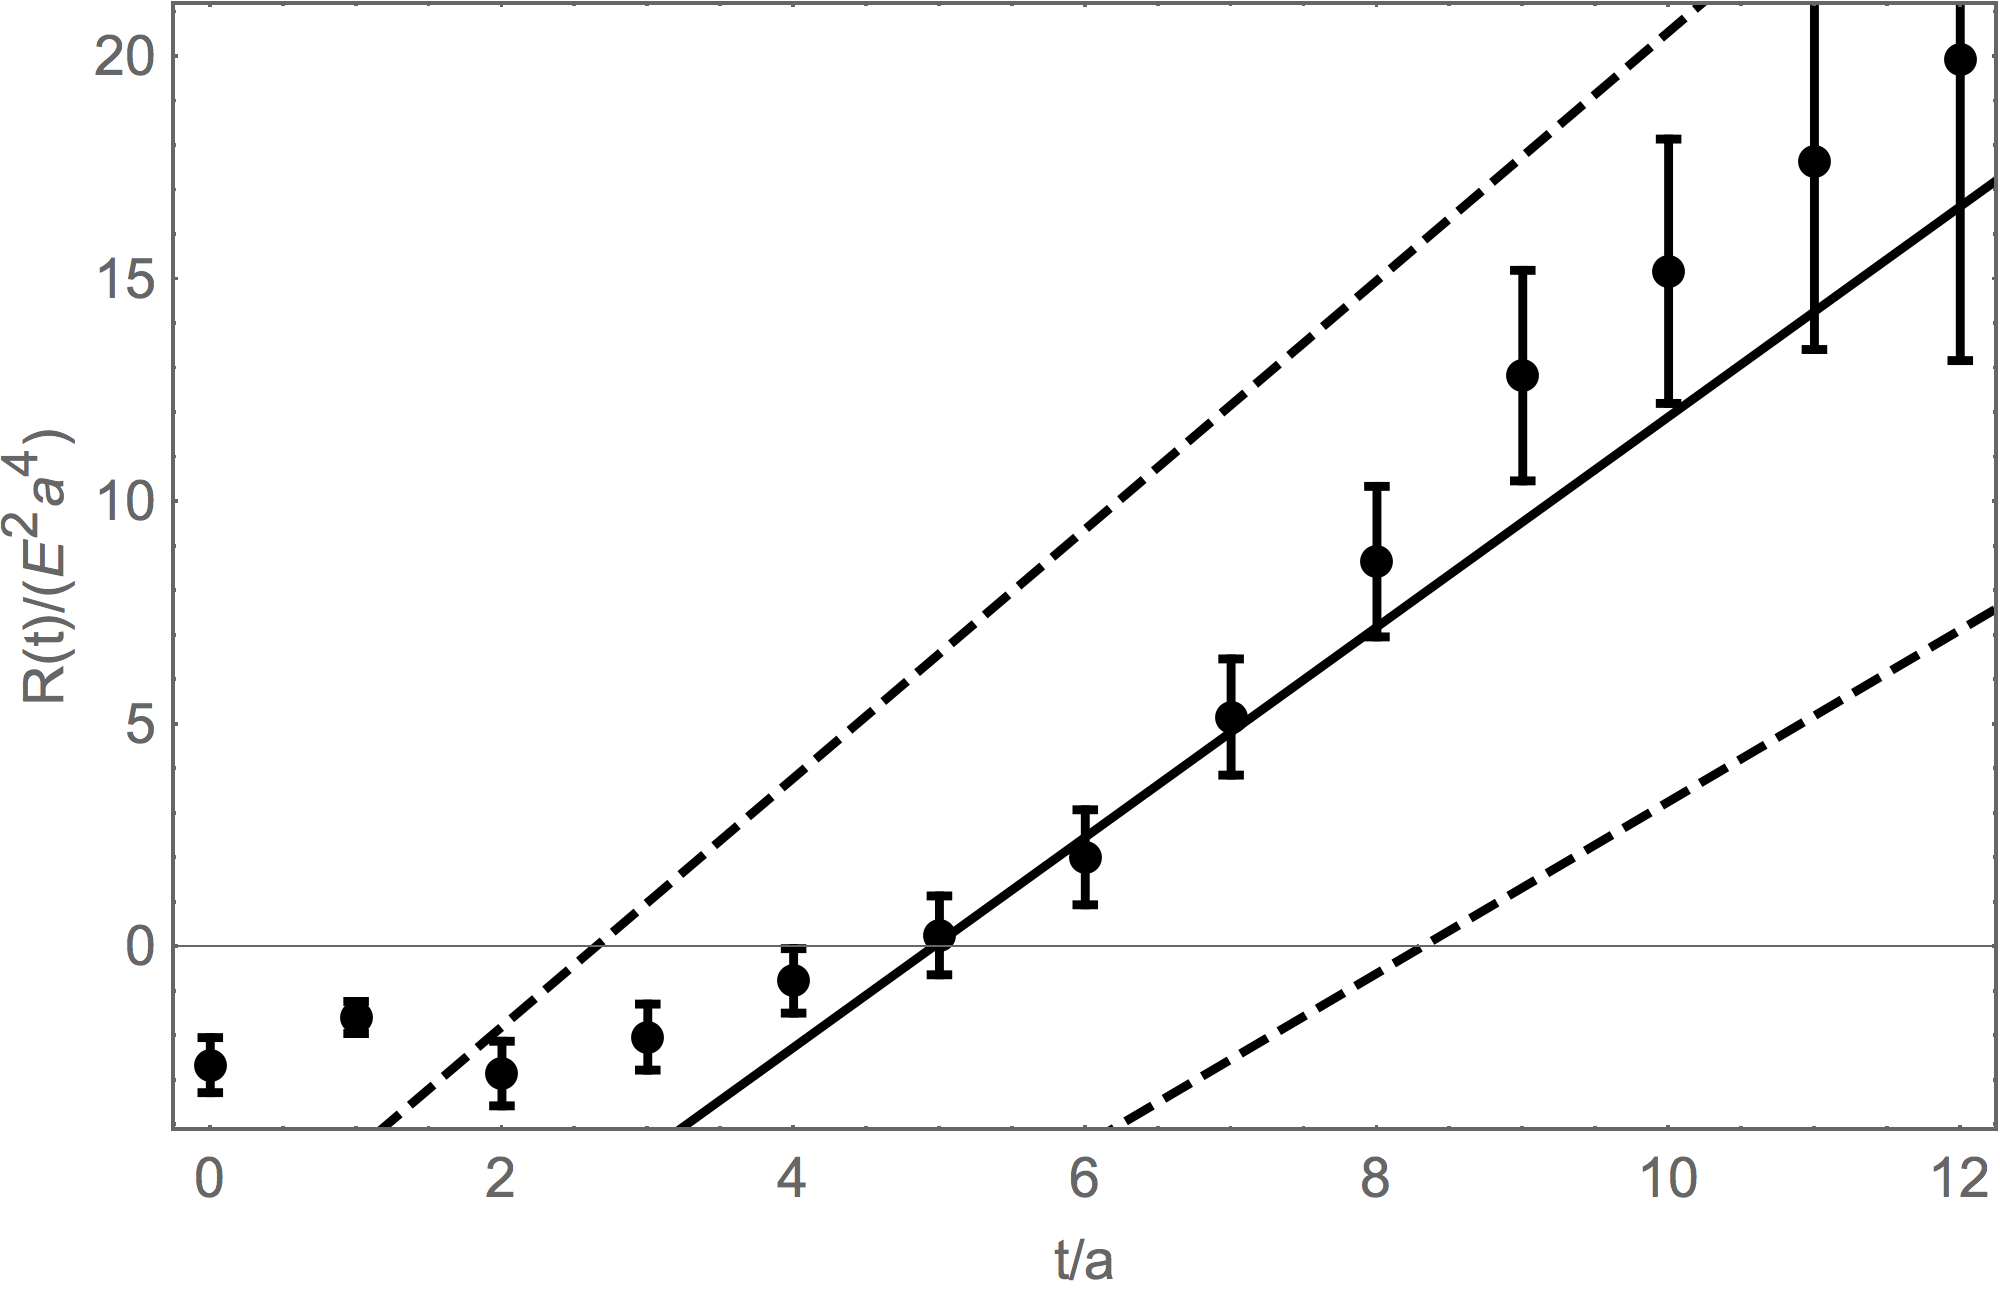
\includegraphics[width=.325\linewidth]{figures/FullshortLineCS.png}\\
\caption{Correlator ratio $R_2(t)$ for all diagrams shown in Figure ~\ref{fig:diagrams}, in units of $E^2a^4$. In these plots, the neutron source was placed at the fixed location $t=0$, and the background field, c.f.~\ref{gauge}, was varied with $t_0=6a$, $t_0=0$, $t_0=-10a$ (from left to right).The dashed lines delimit the linear fit uncertainty in the slope.}
\label{fig:Correlators3wAll}
\end{figure}
%%%%%%%%%%%%%%%%%%%%%%%%%%%%%
%%%%%%%%Generic Cubic Behavior%%%%%%%%%
\begin{figure}[H]
\centering
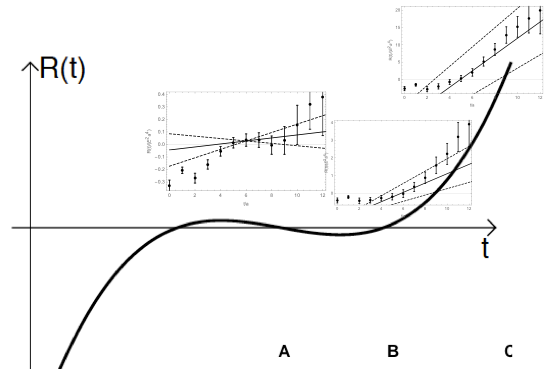
\includegraphics[width=.65\linewidth]{figures/full3window.png}
\\
\caption{3-window generic cubic behavior for all diagrams. The plots in figure~\ref{fig:Correlators3wAll} 
are the three time windows shown here in their approximate positions.}
\label{fig:CubicAll}
\end{figure}
%%%%%%%%%%%%%%%%%%%%%%%%%%%%%

%%%%%Full EXTREMUM TABLE%%%%%%
\begin{table}[H]
\begin{center}
    \begin{tabular}{ | l | l| l | l |}
    \hline
     Fit range [$t/a$] 			& 5 to 7   		& 4 to 8   		& 3 to 9  \\ \hline
     Inflection point [$t/a$]		&  6.99(39)   	&  6.97(38)    	& 7.12(34)    \\ 
     						& 6.90(87)		& 7.12(91)		& 7.7(1.0)	\\ \hline
     Extremal slope [$a^3$]		&   -0.002(24)   & 0.001(19)   	& 0.005(16)  \\
     						& -0.006(61)	& -0.023(50)	& -0.037(46) \\ \hline
    \end{tabular}
\end{center}
\caption{Inflection points and extremal slopes for the $\chi^2$ linear fits in the 3-window analysis with parabola minimum lift correction, for all connected and disconnected diagrams. \todo{results from reduced statistics are given in the lower lines}}
\label{tab:ExtremaMultiPointAll}
\end{table}
%%%%%%%%%%%%%%%%%%%%
%%%%%%%%%%%%%%%%%%%%%%%%%
The electric polarizability for all diagrams was calculated from 
the results in table~\ref{tab:ExtremaMultiPointAll}
for the selected fitting ranges, with and without the Foldy-Wouthuysen contribution.
Table~\ref{tab:FullPolarizabilities} shows the electric polarizability 
measurements for the ``multi point" dataset.

%%%%%%%%%%All diagramsPolarizability 10^-4 fm^3%%%%%%
\begin{table}[H]
\begin{center}
    \begin{tabular}{|l|l|l|l|}
    \hline
     Fitting range ($t/a$) 						&  5 to 7 	&  4 to 8 	& 3 to 9	\\ \hline
     $\alpha_E$ [$10^{-4}$ $\text{fm}^3$]   			& 0.07(92)	&-0.04(72)& 0.19(72) \\
     										&	&	&  \\ \hline
     $\alpha_E-\alpha_{FW}$ [$10^{-4}$ $\text{fm}^3$] 	& 0.29(92)	&-0.19(63)& 0.04(63) \\ 
 										&	&	&	\\ \hline
    \end{tabular}
\end{center}
\caption{Static electric polarizability  $\alpha_E$ and static electric polarizability minus Foldy-Wouthuysen contribution $\alpha_E-\alpha_{FW}$ from the extremal values (all diagrams, $\chi^2$ fits, ``multi point" dataset) of the three fitting ranges in units of $10^{-4}$ $\text{fm}^3$. \todo{'point' results?}}
\label{tab:FullPolarizabilities}
\end{table}
%%%%%%%%%%%%%%%%%%%%%%%%%%%%%
